En la figura \ref{fig:ej6-1} se ilustra el mismo lote que en el punto anterior, pero ahora usando el \emph{scheduler FCFS}.

\begin{figure}[H]
  \centering
  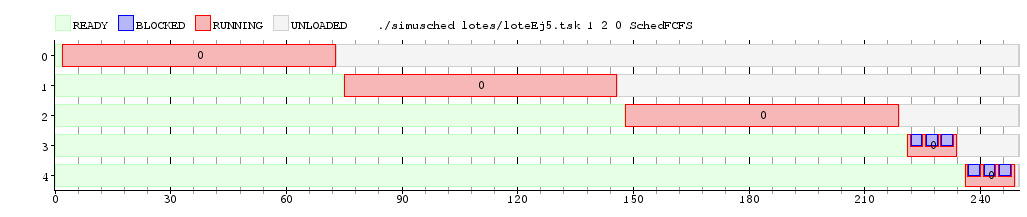
\includegraphics[width=1\textwidth]{img/imgEj6-1}
  \caption{}
  \label{fig:ej6-1}
\end{figure}

Una de las diferencias entre ambos schedulers es que el tiempo total que se requiere para ejecutar todo el lote es siempre menor con una estrategia FCFS. Esto se debe a que este algoritmo de \emph{scheduling} realiza la mínima cantidad de cambios de contexto posibles (uno por cada proceso involucrado).

Al mismo tiempo empeora mucho la latencia de las tareas respecto a \emph{Round Robin}. Además, con FCFS, esta métrica depende fuertemente del orden de llegada de los procesos, pues hay una gran diferencia entre que lleguen las tareas en orden creciente de tiempo de ejecución (mejor caso), y lo opuesto (peor caso, figura \ref{fig:ej6-1}). En ese sentido, \emph{Round Robin} es más robusto pues la latencia de los procesos depende mucho menos del orden de llegada y más de la duración del \emph{quantum} (lo que resulta mucho más manejable). 

En la figura \ref{fig:ej6-2} se grafica el mismo lote de tareas para FCFS pero cambiando el orden de llegada por el de mejor caso. Una buena forma de notar la diferencia en las latencias respecto del gráfico \ref{fig:ej6-1} es comparar la latencia del proceso con máxima latencia de cada gráfico, es decir el último en ejecutar en cada caso.

\begin{figure}[H]
  \centering
  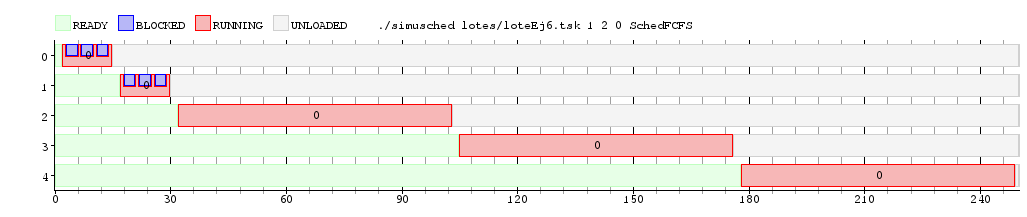
\includegraphics[width=1\textwidth]{img/imgEj6-2}
  \caption{}
  \label{fig:ej6-2}
\end{figure}

